\documentclass[a4paper, 11pt]{letter}

\usepackage[brazil]{babel}
\usepackage[utf8]{inputenc}
\usepackage[T1]{fontenc}
\usepackage[sc]{mathpazo}
\usepackage{inconsolata}
\usepackage{graphicx}

\usepackage{geometry}
% \geometry{lmargin=3cm, rmargin=3cm, tmargin=4cm, bmargin=4cm}

\usepackage{background}
\backgroundsetup{%
  scale = 1,       %% change accordingly
  angle = 0,       %% change accordingly
  opacity = 0.30,  %% change accordingly
  color = black,   %% change accordingly
  contents = {
    \begin{tikzpicture}[remember picture, overlay]
      \node[yshift = 2cm, xshift = 0pt] at (current page.center) {
        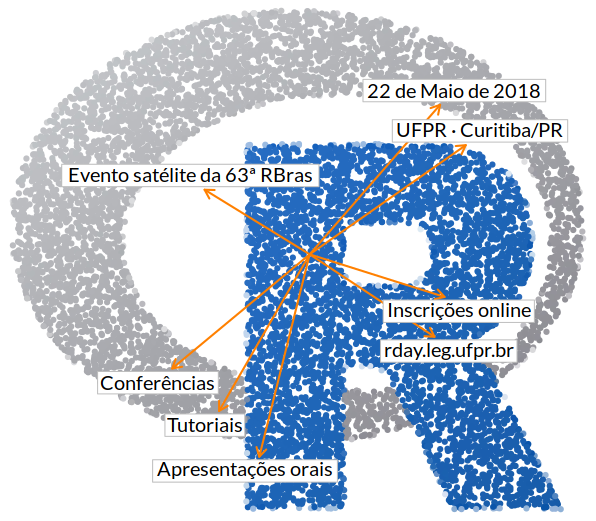
\includegraphics[width = 0.7\textwidth]{r-day.png}};
        % 
\includegraphics[width = 0.6\textwidth]{leg.pdf}};
    \end{tikzpicture}}
}

% \usepackage[onehalfspacing]{setspace}
\usepackage{setspace}
\linespread{1.5}

\usepackage{fancyhdr}
% \addtolength{\headheight}{\baselineskip}
\renewcommand{\footrulewidth}{0.5pt}

\pagestyle{fancy}
\headsep = 2cm  % espaço entre header e texto
\lhead{
\includegraphics[height=50pt]{../prova-ufpr/ufpr_logo.png}}
\rhead{
\includegraphics[height=50pt]{leg.pdf}}
\chead{\footnotesize \bf
  % MINISTÉRIO DA EDUCAÇÃO \\
  UNIVERSIDADE FEDERAL DO PARANÁ \\
  SETOR DE CIÊNCIAS EXATAS \\
  DEPARTAMENTO DE ESTATÍSTICA\\
  LABORATÓRIO DE ESTATÍSTICA E GEOINFORMAÇÃO}
\cfoot{}

\date{}

\def\DATA{..hoje..}
\def\CARTATIPO{..cartatipo..} % {0: comp. inscrição, 1: ac. submissão}
\def\AUTOR{..autor..}         % Nome do autor.
\def\TITULO{..titulo..}       % Título do trabalho, quando houver.
\def\FECHAMENTO{Atensiosamente,}

\def\COMPLEMENTO{
  no \textbf{R Day}: Encontro nacional de usuários do R que será
  realizado em Curitiba no dia 22 de Maio de 2018.  Os horários e
  instruções para a apresentação das atividades serão divulgados na
  \textit{homepage} do evento oportunamente em
  \textit{http://rday.leg.ufpr.br}.
}

%=======================================================================

\begin{document}

\begin{letter}{}

  \hfill \DATA \vspace{1em}

  \ifx\CARTATIPO\undefined % -------------------------------------------
  CARTA-TIPO-NULL
  \else
  \if\CARTATIPO1
  % CARTA PARA ACEITE DE TRABALHO --------------------------------------
  \begin{center}
    \uppercase{Carta de Aceite de Submissão}
  \end{center}

  \opening{\AUTOR,}

  \vspace{1em}

  \hspace{1.5cm}
  É com satisfação que comunicamos que a sua submissão intitulada
  ``\textbf{\TITULO}'' foi aceita para apresentação \COMPLEMENTO

  \else
  % CARTA PARA RECIBO DE INSCRIÇÃO -------------------------------------

  \begin{center}
    \uppercase{Comprovação de Inscrição}
  \end{center}

  \opening{Aos interessados,}

  \vspace{1em}

  \hspace{1.5cm}
  Atestamos que \textbf{\AUTOR} está inscrito \COMPLEMENTO

  \fi
  \fi

  \vspace{2em}
  \hspace{1.5cm} \FECHAMENTO
  \vspace{2em}

  % Isso tem que estar depois de \opening{} para que seja aplicado.
  \pagestyle{fancy}
  \thispagestyle{fancy}

  % Primeira assinatura.
  \begin{minipage}[b]{0.45\linewidth}

    \vspace*{2em}
    \centering{\includegraphics[scale = 0.9]{/home/walmes/Dropbox/RevoLEG/sign-fernando-mayer.png}}
    % \centering{\tikz{\draw[dashed] (0, 0) rectangle node {SUA ASSINATURA AQUI} (6, 4);}}
    \vspace*{-6em}

    \begin{flushright}
      \rule{\textwidth}{0.5pt}

      Prof. Fernando de Pol Mayer\newline
      Lab. de Estatística e Geoinformação\newline
      Coordenador do R Day\newline
    \end{flushright}

  \end{minipage}
  \hfill
  \begin{minipage}[b]{0.45\linewidth}

    \vspace*{2em}
    \centering{\includegraphics[scale = 0.9]{/home/walmes/Dropbox/RevoLEG/sign-walmes-zeviani.png}}
    % \centering{\tikz{\draw[dashed] (0, 0) rectangle node {SUA ASSINATURA AQUI} (6, 4);}}
    \vspace*{-4em}

    \begin{flushright}
      \rule{\textwidth}{0.5pt}

      Prof. Walmes Marques Zeviani\newline
      Lab. de Estatística e Geoinformação\newline
      Vice-coordenador do R Day\newline
    \end{flushright}

  \end{minipage}

  \vfill

\end{letter}

\end{document}
